\section{Metodología}
La metodología para el desarrollo del controlador de vuelo para un UAV de ala fija se puede observar en 
 la figura \ref{fig:diagrama metodo}, en esta figura se observa la estructuración del proyecto en varias etapas, desde la investigación inicial hasta la prueba de vuelo. Comienza con la investigación y la creación de un diagrama funcional, seguido del desarrollo del hardware, el enclosure electrónico, el firmware y la interfaz de usuario. El hardware incluye el diseño y la fabricación electrónica del controlador de vuelo, mientras que el enclosure electrónico es el encargado de dar soporte y protección al circuito. Finalmente, el firmware abarca la adquisición de datos, telecomunicaciones y control de actuadores, y la interfaz se encarga de la visualización de dichos datos. Tanto el firmware como la interfaz de usuario se revisan para asegurar su correcto funcionamiento. Finalmente, se realizan pruebas locales y de vuelo para validar el sistema completo.

\begin{figure}[H]
    \centering
    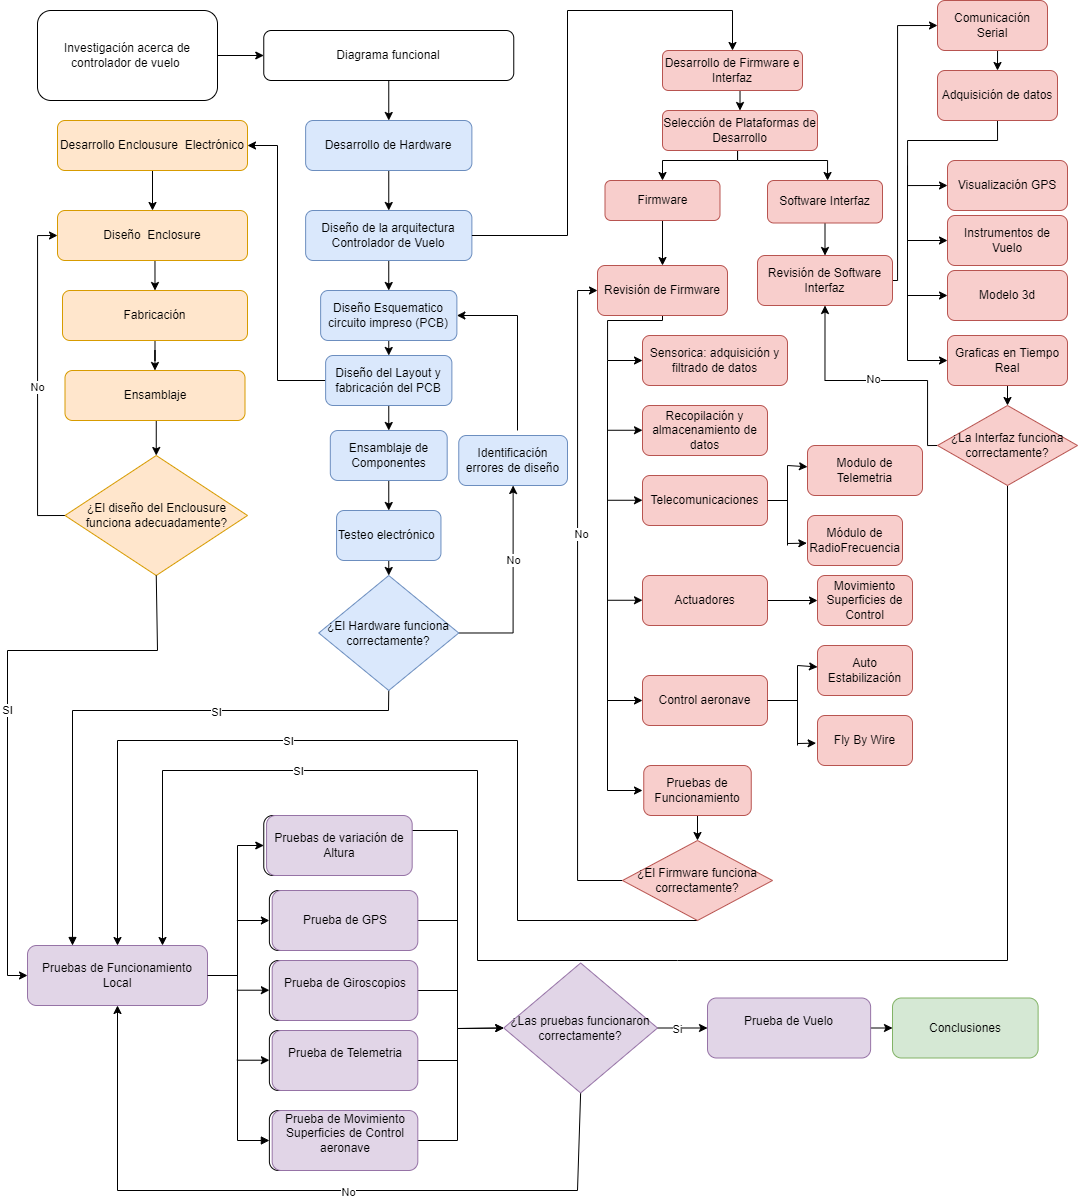
\includegraphics[width=14 cm]{Imagenes/Metodologia/metodologia.png}
    \caption{Diagrama Metodología Implementada}
    \label{fig:diagrama metodo}
\end{figure}

\clearpage
\section{Diagrama Funcional}
En la figura \ref{fig:bloques} se muestra el diagrama funcional de un controlador de vuelo de UAV de ala fija, este incluye los siguientes componentes esenciales: un barómetro para el cálculo de la presión atmosférica, una unidad de movimiento inercial para calcular la orientación, y un módulo GPS para la localización. Un procesador central que analiza los datos de estos sensores y ejecuta los algoritmos de control. Así mismo una forma de controlar los servomotores, que forman parte del sistema de control de actuadores de vuelo, implementando las órdenes del procesador para manejar los alerones, timón, elevadores y el sistema de propulsión. La unidad de alimentación eléctrica provee la energía necesaria para todos los componentes. Un módulo de telemetría y un módulo de enlace por radiofrecuencia que permiten la transmisión y recepción de datos, facilitando la supervisión y el  control remotamente. Finalmente, una unidad de visualización de datos críticos en tiempo real y una unidad de almacenamiento que registra la información relevante del vuelo.
\begin{figure}[H]
    \centering
    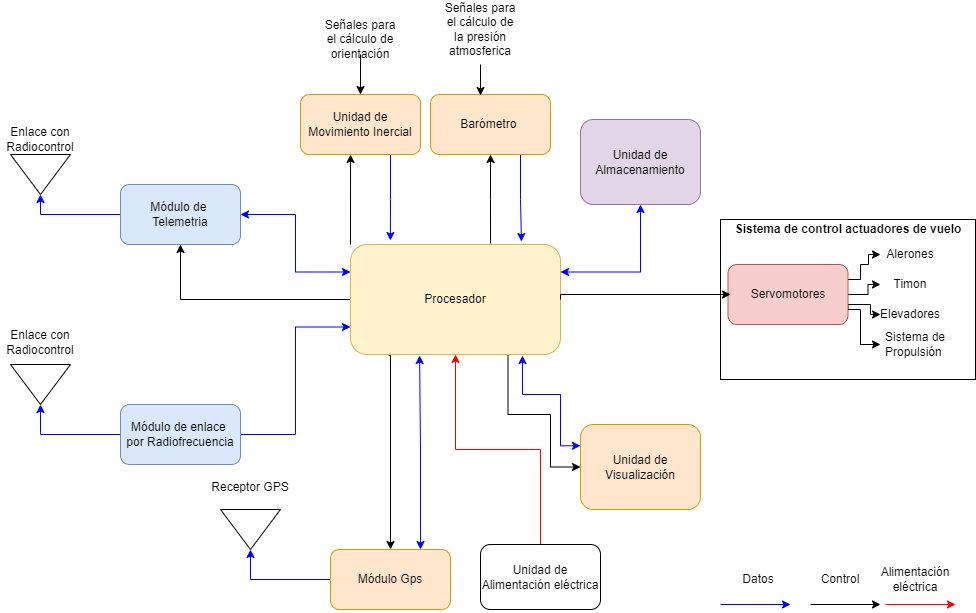
\includegraphics[width=\textwidth]{Imagenes/funcional/Diagrama funcional.png}
    \caption{Diagrama de bloques del Controlador de Vuelo para UAV de ala fija }
    \label{fig:bloques}
\end{figure}







